\chapter{Datacenter}
10 years ago datacenters were no more than a room with some computers, air conditioners and some plugs to power up the devices.
Later on, customers started asking server vendors to include in the servers utilities to allow an \textit{automated datacenter management}.
Thus the trend moved towards \textbf{\ul{Software Defined Datacenter}}, which currently is the only possible way to deploy a Datacenter.

An \textbf{Active Datacenter} allows for internet storage (?)

A Datacenter should be \textbf{future-proof}: servers may be replaced, but updating a whole datacenter is at least a 1-year project.

\section{Structure}
\textit{Racks} are made of ---$\sim 42$--- \textit{units}.

Besides server theirselves, there is a \textbf{cooling system}.
The first issue is the how to provide cool air. Then there is also how to define an evacuation plan, which must take into account dust.

However also the \textbf{floor} is not to be negliged.
\begin{itemize}
   \item \textit{Floating} floor or Ground floor
   \begin{itemize}
      \item 
      \note{
         \textit{``A “floating floor” in a data center, also known as a “raised floor”, is a type of construction used in data centers to create a void between the actual concrete floor and the floor tiles where the servers and other equipment are located12. This space is typically used for routing cables and for air circulation, which helps with cooling the equipment1."}\footnote{ChatGPT 4.0 - Generated}
      }
   \end{itemize}
   \item \textit{Resistance} usually around $1 \frac{ton}{m^2}$  
\end{itemize}

For example, in San Piero A Grado, there was a power cabin receiveing current from three lines.
Now the whole power management components are in a container outside the building placed close to the facility.

Cables are not super-resistant to current. A lot of current passing through a copper wire will \textit{exhaust} both the wire and the components receiving such current;
hence the current should also be balanced among different cables, to avoid exhausting some components before the others.


A UPS ---first of all--- stabilizes the output current.

In theory $1V * 1A = 1W$, but in reality, performing such conversion \ul{something gets lost}, so we have
\[I * V * cos \phi = W\]

\section{Power Management}

Electric panels (aka \textit{switchboards}) allow segmenting the power supply in the various zones of the datacenter.

\textbf{PDU}s stands for \textit{Power Distribution Units}, and allow to distribute power for a server units in a rack.
Typically, for each PDU there is another one, providing redundacy and thus resilience/robustness.

\nl

\begin{definition}[PUE]
\textit{Power Usage Effectiveness} \textbf{PUE} measures the efficiency of a Datacenter.
\[PUE = \frac{
   \textit{Total energy}
}{\textit{ICT energy}}\]
\end{definition}
The \ul{reason for improving Datacenter design is to lower the PUE};
basically to save money, but also for ``green-environment'' concerns.

\begin{center}
   But \textit{\ul{when}} should PUE be measured?
\end{center}
The PUE in January is very different from the one in August, so generally it is calculated as the average of one year.

Note that a poorly designed datacenter placed in Siberia with $-20^{\circ}$ may have a lower PUE than a datacenter in Italy, for instance.\\
In particulare geographical zones with high temperature variations over the year (e.g. in Italy the temperature variates from 40 to 50 Celsius degrees), are strongly unrecommended to build datacenters in.
\ul{A counterintuitive example is the desert}, where the temperature is very high during the day and very low during the night, but in general the temperature over the year is \textbf{stable}; allowing for defining physical processes exploiting such stability.\\
Also the oceans have a very stable temperature; not on the surface, but deep down it is very stable.

\section{Cooling}
Note that racks are always placed back-to-back, because the front requires cool air, and the back outputs hot air.
\section{CRAC}
\begin{figure}[htbp]
   \centering
   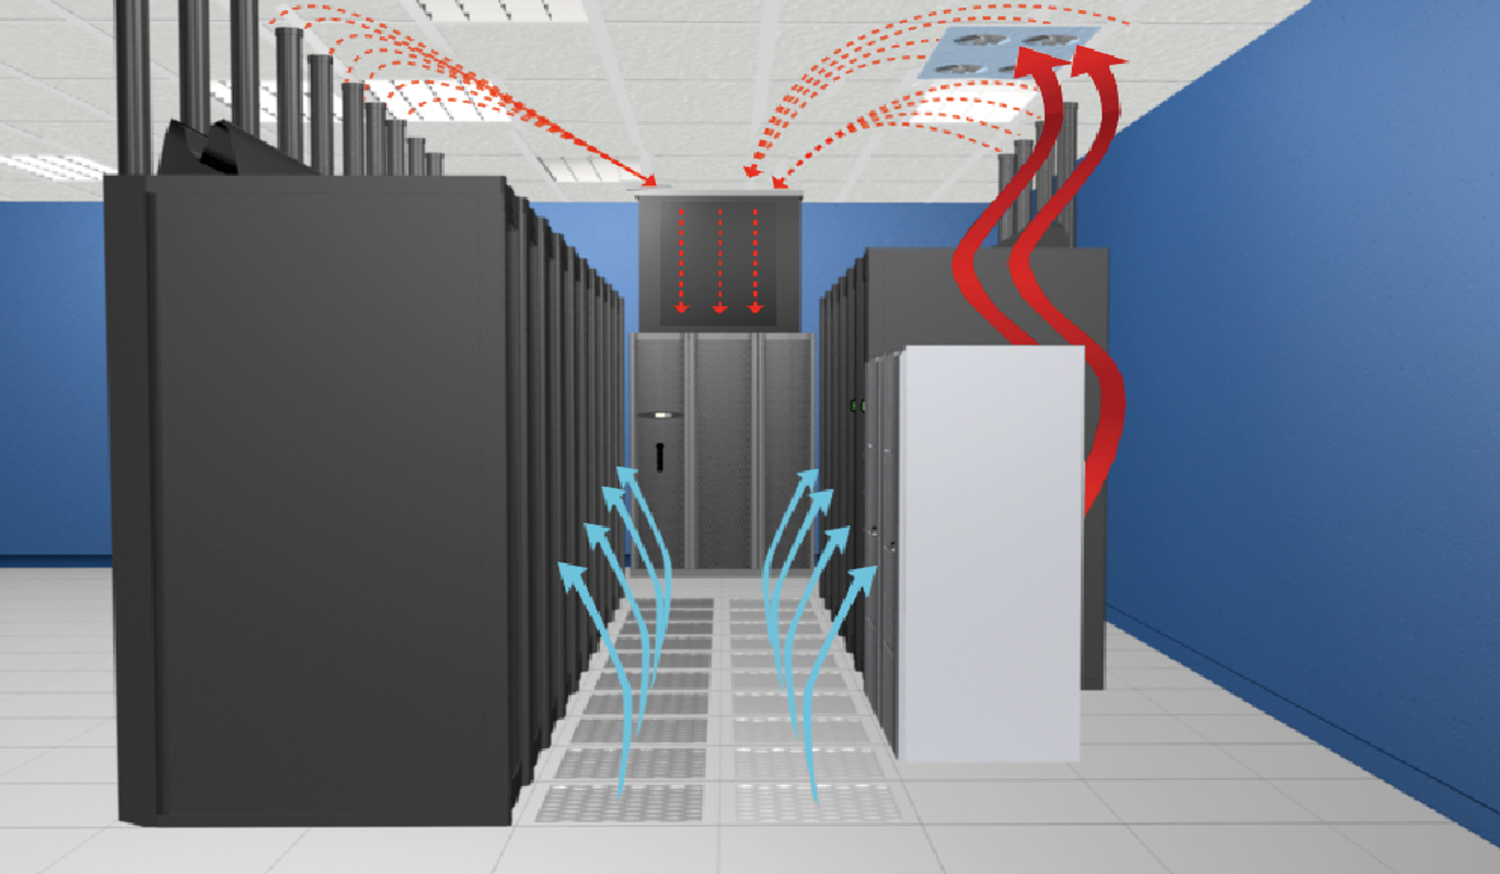
\includegraphics{images/CRAC.jpg}
   \caption{CRAC/CRAH cooling architecture}
   \label{fig:CRAC}
\end{figure}
Chillers take hot air from above and push cool air in the bottom. Then air pushed under the floating floor wants to exit, and does so going through the grates placed in front of the racks.
The racks suck the cool air in front and output hot air from the back.

{
   There are two \textbf{drawbacks}:
   \ns
\begin{enumerate}
   \item It is difficult to confine and keep separated hot air and cool air. The mixup between the two leads to cooling inefficiency, thus energy and money waste
   \item In case a rack has a workload heavier than others and thus requires more cooling air, the chiller must provide more cool air to all the racks in the same row;
   this makes this architecture particularly inefficient for datacenter which have heterogeneous workloads.
\end{enumerate}
}

\newpage
\section{Inrow Cooling}
\begin{paracol}{2}
   \colfill
   The fan ``towers'' are called \textit{inrow cooling}.

   The first advantage is that it allows for heterogeneous cooling in the datacenter.
   Secondarily, a fan outputs hot air directly where another fan expects it to be.
   This allows to confine hot air and to avoid wasting energy in outputting air and sucking it.

   \colfill
   \switchcolumn
\begin{figure}[htbp]
   \centering
   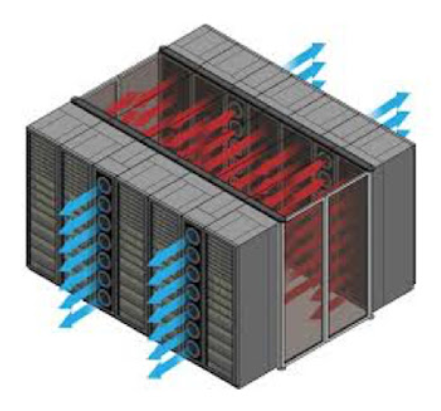
\includegraphics{images/inrow_cooling.png}
   \caption{Inrow cooling architecture}
   \label{fig:inrow_cooling}
\end{figure}
\end{paracol}